
% C:IKNP03 https://www.iacr.org/archive/crypto2003/27290145/27290145.pdf
% Nie07  "Extending Oblivious Transfers Efficiently How to get Robustness Almost for Free"
% C:KelOrsSch15  https://eprint.iacr.org/2015/546.pdf
% RSA:OrrOrsSch17  https://eprint.iacr.org/2016/933.pdf
% EC:ALSZ15 https://eprint.iacr.org/2015/061.pdf


\section{OT Extension} \label{sec:otext}


In this section we explore the rich implications Endemic OT has on efficient 1-out-of-$N$ OT extension along with presenting three new attacks and fixes of existing OT extension protocols\cite{C:KelOrsSch15, RSA:OrrOrsSch17} with Uniform Message security\footnote{\cite{C:KelOrsSch15, RSA:OrrOrsSch17} refer to uniform OT as random OT $\mathcal{F}^{m,\kappa}_{\textsf{ROT}}$}. These protocols are derived from the seminal black-box protocol of Ishia, Kilian, Nissim and Petrank\cite{C:IKNP03}. We note that in all cases the Sender Chosen Message variant of these protocols\cite{C:IKNP03, C:KelOrsSch15, RSA:OrrOrsSch17} are secure. %In particular, these Sender Chosen Message protocol perform the following transformations $\OOT^\send\overset{\pi_1}{\rightarrow} \OOT^\E \overset{\pi_2}{\rightarrow} \OOT^\send$. However, as we will explore later, \figureref{fig:OTExtrelations} suggestions that a more efficient transformation exists where $\pi_1$ takes $\OOT^\E$ as input, e.g. a two round extension protocol satisfying $\OOT^\rec$.



The functionality of 1-out-of-$N$ OT extension allows $\nc\approx\kappa$ instances of 1-out-of-2 OTs to be transformed into $m=\textsf{poly}(\kappa)$ instances of 1-out-of-$N$ OTs. There are several advantages of this transformation 1) $m$ can be polynomial times larger than $\nc$. 2) Only symmetric key cryptography is required which provides a larger performance improvement. 3) In some cases $N$ can be exponential in the security parameter $\kappa$. The 1-out-of-2 OTs that are being transformed are referred to as \emph{Base OTs}. Existing protocols\cite{C:IKNP03,EC:ALSZ15, C:KelOrsSch15, RSA:OrrOrsSch17} have called for the use of base OTs with the Sender Tweakable Message Security notion, e.g. $\OOT^\send$. However, this requirement can be relaxed to allow the base OTs to only achieve Endemic security. As shown by \figureref{fig:OTExtrelations}, in both cases ($\OOT^\send$ or $\OOT^\E$ base OTs) the OT extension protocol outputs messages that satisfy the Endemic security notion.  Tradition OT extension protocols, e.g. \cite{C:IKNP03,EC:ALSZ15, C:KelOrsSch15}, then apply the $\Pi^{\send}_{1,N}$ transform from \figureref{fig:protoSendOT} to realize the Sender Chosen Message functionality $\OOT^\send$. This observation suggests that more efficient OT extension can be realized by replacing Sender Chosen Message base OTs with Endemic OTs, e.g. our protocol.

In addition, the authors of \cite{C:KelOrsSch15,RSA:OrrOrsSch17} suggest that the $\Pi^{\send}_{1,N}$ transform that was originally specified by \cite{C:IKNP03} can be removed and resulting protocol would satisfy the Uniform Message security notion. However, as previously stated, we show this not to be the case and that the protocol only achieve Endemic security. We note that many protocols that utilize Uniform Message security can likely tolerate the weaker notion of Endemic security, e.g. \cite{EC:RinRos17,CCS:RinRos17}.  However, other protocols such as the set inclusion protocol of \cite[Figure 5]{RSA:OrrOrsSch17} are insecure\footnote{The sender set all the OT messages to be the same value and force the receiver to conclude their item is in the sender's set.} when Uniform Message security is not satisfied. 

Uniform Message security can be achieved in several ways. One solution is the the black-box transformation $\Pi^\U_{1,N}$ of \figureref{fig:uniformOT} which lifts an OT protocol with Endemic security to satisfy Uniform Message security. However, this would require additional rounds and significant communication. We demonstrate an alternative solution which replaces the base OTs with a protocol that satisfies Uniform Message, Uniform Selection security $\OOT^{\U u}$ and prove that this yields an OT extension protocol with Uniform Message security without the need to modify the extension protocol. More generally, \figureref{fig:OTExtrelations} shows the relation between different base OT security notions and the resulting OT extension message security. For example, the protocols of \cite{C:IKNP03,EC:ALSZ15, C:KelOrsSch15} perform
$$
\OOT^\send \xrightarrow{\Pi^{\textsf{ext}}} \OOT^\E \xrightarrow{\Pi^{\send}_{1,2}} \OOT^\send
$$
where $\Pi^\textsf{ext}$ is their respective extension protocol up to hashing.

\begin{figure}[h!]
	\centering
	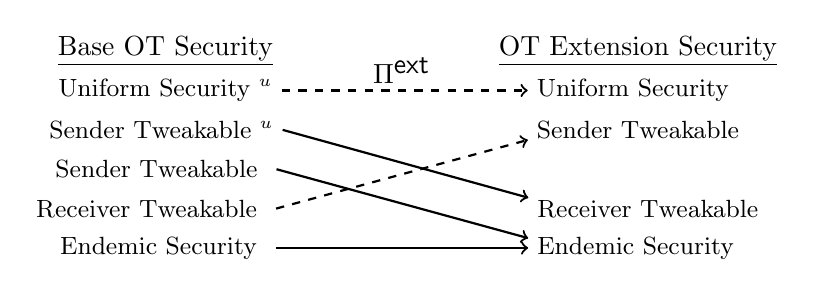
\begin{tikzpicture}[scale=0.5]\small
	\node (pi) at (6,4.5) {\normalsize $\Pi^\textsf{ext}$};
	\node (Base) at (0,5) {\underline{\normalsize Base OT Security}};
	\node (U) at (0,4) {Uniform Security $\OOT^{\U u}$};
	\node (SCu) at (-0.1,3) {Sender Tweakable $\OOT^{\send u}$};
	\node (SC) at (-0.1,2) {Sender Tweakable $\OOT^{\send}$};
	\node (RC) at (-0.35,1) {Receiver Tweakable  $\OOT^{\rec}$};
	\node (E) at (-0.05,0) {Endemic Security  $\OOT^{\E}$};
	
	
	\node (Ext) at (12,5) {\underline{\normalsize OT Extension Security}};
	\node (EU) at (12,4) {Uniform Security $\OOT^{\U}$};
	\node (ESC) at (12.13,3) {Sender Tweakable $\OOT^{\send}$};
	\node (ERC) at (12.38,1) {Receiver Tweakable  $\OOT^{\rec}$};
	\node (EE) at (12.07,0) {Endemic Security  $\OOT^{\E}$};
%	\draw [-implies,double equal sign distance] (U) -- (SC);
%	\draw [-implies,double equal sign distance] (U) -- (RC);
%	\draw [-implies,double equal sign distance] (SC) -- (E);
%	\draw [-implies,double equal sign distance] (RC) -- (E);
	\draw [->, thick, dashed] (U) -- (EU);
	\draw [->, thick] (E) -- (EE);
	\draw [->, thick] (SCu.east) -- (ERC.175);
	\draw [->, thick, dashed] (RC.east) -- (ESC.185);
	\draw [->, thick] (SC.east) -- (EE.175);
	
%	\draw [-, thick] (5,2.5)-- (TC);
%	\draw [->, thick] (E) .. controls (1,0.75) .. (SC);
%	\draw [->, thick] (E) .. controls (7,0.75) .. (RC);
	\end{tikzpicture}
	\label{fig:OTExtrelations}
	\caption{
		The figure depicts the implication different Base OT security notions (\definitionref{def:otSec}) have on the result OT extension protocol.  $A\rightarrow B$ denotes that any OT realizing security $A$ can be efficiently transformed by $\Pi^\textsf{ext}$ into an OT extension realizing security $B$, where $\Pi^\textsf{ext}$ is the protocol of \figureref{fig:otExt} such that $\OOT$ is the left hand side oracle. The dashed arrows are the same expect $\Pi^{\textsf{ext}}$ must be slightly modified. 
	}
\end{figure}










Next we review the OT extension protocol of \cite{RSA:OrrOrsSch17} which we describe in \figureref{fig:otExt}. The base OTs are performed on inputs that are sampled uniformly at random where the roles of the sender and receiver are reversed with respect to the OTs that are output by the extension. That is, \send will receiver $(b_j, \tt^j_{b_j})\in\mathbb{F}_2\times \mathbb{F}_2^m$ while $\rec$ will receive $(\tt^j_0,\tt^j_1)\in\mathbb{F}_2^m\times \mathbb{F}_2^m$ for $j\in[\nc]$.

\rec forms two matrices $T_0,T_1\in \mathbb{F}_2^{m\times \nc}$ by concatenating the base OT messages as column vectors, i.e. $T_i:=(\tt^1_i ... \tt^\nc_i)$. Similarly, \send forms the matrix $T_{\text{\textbf{b}}}:=(\tt^1_{b_1}...\tt^\nc_{b_\nc})$. \rec then encodes their 1-out-of-$N$ selections $\ww_1,...,\ww_m$ into a matrix $C\in \mathbb{F}_2^{m\times \nc}$. Each row $\cc_i$ is the codeword $\mathcal{C}(\ww_i)$ of \rec's $i$-th selection $\ww_i\in [N]$, $\mathcal{C}$ is a binary code of length $\nc$, dimension $\kc=\log_2\kappa$ and minimum distance $\dc\geq\kappa$. \rec sends the matrix
$$
	U=T_0+T_1+C
$$
to \send. Observe that $U$ encodes the selections of \rec but the selection is perfectly masked/encrypted due to the $j$-th column of $U$ being masked by the column $\tt^j_{1-b_j}$ which is uniformly distributed in the view of \send. Upon receiving $U$, \send computes $Q\in\mathbb{F}^{m\times\nc}$ where the $j$-th column is defined as $\qq^j:=b_j\cdot \uu^j+\tt^j_{b_j}=b_j\cdot \cc^j+\tt^j_0$. It holds that 
$$
	\qq_i=\cc_i\odot \bb + \tt_i
$$
where $\tt_i,\qq_i$ is the $i$-th row of $T_0,Q$, respectively, and $\bb:=(b_1,...,b_\nc)\in \mathbb{F}^\nc_2$. \rec will output $\vv_{i,\ww_i}:=\H(i, \tt_i)$. \send can then generate any OT message by computing $\vv_{i,\ww}:=\H(i, \qq_i + \mathcal{C}(\ww)\odot \bb)$. Correctness of this operation follows from 
\begin{align*}
	\qq_i + \mathcal{C}(\ww)\odot \bb =&  (\mathcal{C}(\ww_i)\odot \bb + \tt_i) + \mathcal{C}(\ww)\odot \bb\\
	=& (\mathcal{C}(\ww_i) + \mathcal{C}(\ww)) \odot \bb +\tt_i.
\end{align*}
Let $\delta = \mathcal{C}(\ww_i) + \mathcal{C}(\ww)$. In the event that $\ww_i=\ww$, then $\delta=0$ and \send computes the same $\vv_{i,\ww_i}$ value as \rec. Otherwise the hamming distance $\textsf{HD}(\delta)\geq \dc\geq \kappa$ by construction of $\mathcal{C}$. For $\rec$ to generate any other OT message $\vv_{i,\ww}$ s.t. $\ww\neq \ww_i$, \rec must guess the value $\delta\odot \bb\in \mathbb{F}^\nc_2$ given $\delta$, which takes time $2^{\textsf{HD}(\delta)}=O(2^\kappa)$.

To realize the ideal Sender Chosen Message oracle $\OOT^\send$ \cite{C:IKNP03,EC:ALSZ15,C:KelOrsSch15,RSA:OrrOrsSch17} specify two additional steps:
\begin{enumerate}

	\item A proof that all rows in $C$ can be decoded. Ishai et al. \cite{C:IKNP03} proposed a cut-and-choose approach while the more recent schemes \cite{C:KelOrsSch15,RSA:OrrOrsSch17} improve on the efficiency of these proofs by making \rec send random linear combinations of $\tt_i,\ww_i$ and having \send check they are consistent with same combination of $U$. We defer the details behind these proofs to \cite{C:KelOrsSch15,RSA:OrrOrsSch17}.
	
	\item The parties apply the Sender Chosen OT transformation $\Pi^{\send}_{1,N}$ from \figureref{fig:protoSendOT} which reduces sender chosen to endemic OT. That is, \send must send their chosen messages $(x_{i,1},...,x_{i,N})_{i\in [m]}$ encrypted under the corresponding key $(\vv_{i,1},...,\vv_{i,N})_{i\in [m]}$, e.g. \send sends $e_{i,j}:=x_{i,j}+\vv_{i,j}$ to \rec who outputs $x_{i,\ww_i}=e_{i,\ww_i}+\vv_{i,\ww_i}$. Note, this step is not included in \figureref{fig:otExt}. Next we will show without this step the protocol only achieves endemic security.
\end{enumerate}




\begin{figure}[t!]
	\vspace{-1cm}
	\framebox{\begin{minipage}{0.95\linewidth}\small
			\textsc{Parameters:} $\kappa$ is the computational security parameter. $m$ denotes the number of OTs. $N$ denotes the number of messages each OT has. $\mathcal{C}$ is an $[\nc,\kc,\dc]$ binary linear code such that $\kc=\log_2 N$ and $\dc\geq \kappa$. A bijective map $map : [N]\rightarrow\mathbb{F}^\kc$.\\
			\textsc{Requirements:} $\H : [m] \times \mathbb{F}_2^\nc \rightarrow \mathbb{F}_2^\kappa$ is a random oracle.			
			Let $m'=m+s$ where $s$ is defined in \stepref{step:consistency}. \OOT is an 1-out-of-2 OT oracle with output messages in $\mathbb{F}_2^{m'}$.
			\\
			
			\textsc{Extend:} On input $(\textsc{Extend})$ from \send and $(\textsc{Extend}, (x_1,...,x_m)\in[N]^m)$ from \rec.
			\begin{enumerate}
				\item\label{step:extInit} Both parties invoke $\nc$  instances of $\OOT$  where \send takes the role of the receiver. If $\OOT$ has inputs, the corresponding party  locally samples them uniformly from the input domains. \send receives $(\bb'\in\{1,2\}^\nc, \{\tt^j_{b_j}\}_{j\in [\nc]})$ where $\bb_i=(\bb_i'-1)\in\{0,1\}$. \rec receives $\{(\tt^j_0,\tt^j_1)\}_{j\in [\nc]}$. Let $T_0\in \mathbb{F}^{m'\times \nc}_2$ denote the matrix formed by concatenating the column vectors $\tt^1_0||...||\tt^\nc_0$. \\
				
				%				\item \rec constructs matrices $T_0,T_1\in \mathbb{F}^{m'\times \nc}_2$ from the seeds $\{(\rr^j_0,\rr^j_1)\}_{j\in [\nc]}$ so that the respective columns are:
				%				$$
				%					\tt^j_0 := \PRG(\rr^j_0)\in \mathbb{F}^{m'}_2,\qquad \tt^j_1 := \PRG(\rr^j_1)\in \mathbb{F}^{m'}_2,\qquad \forall j\in[\nc]
				%				$$
				%				In the same way \send produces $\tt^j_{b_j}$, for each $j\in[\nc]$. Summarizing, \rec holds $\{(\tt^j_0,\tt^j_1)\}_{j\in[\nc]}$ and \send holds $\{\tt^j_{b_j}\}_{j\in[\nc]}$.
				%				
				\item\label{step:extSendU} \rec  defines $\ww_i:=map(x_i)$ for $i\in[m]$ and  samples random $\ww_{m+\ell}\gets \mathbb{F}^\kc_2$, for $\ell\in[s]$. Then constructs a matrix $C\in\mathbb{F}^{m'\times \nc}_2$ such that each row $\cc_i$ is the codeword $\mathcal{C}(\ww_i)$. Then, \rec sends to \send the values
				$$
				\uu^j :=\tt^j_0 +\tt^j_1+\cc^j, \qquad \forall j\in[\nc],
				$$
				where $\cc^j$ is the $j$-th column of $C$.
				
				\item\label{step:extCompQ} \send receives $\uu^j\in\mathbb{F}^{m'}_2$ and computes
				$$
				\qq^j := b_j \cdot \uu^j +\tt^j_{b_j} = b_j\cdot \cc^j+\tt^j_0,\qquad \forall j\in[\nc]
				$$
				that form the columns of an $(m'\times \nc)$ matrix $Q$. Denoting the rows of $T_0, Q$ by $\tt_i,\qq_i$, \rec now holds $\cc_i,\tt_i$ and \send holds $\bb, \qq_i$ so that 
				$$
				\qq_i = \cc_i\odot \bb+\tt_i,\qquad \forall i\in[m'].
				$$
				
				\item \emph{Consistency check:}\label{step:consistency} \rec  proves in zero knowledge that given their view $\textsc{view}_\rec$:
				\begin{center}
					$	\forall i\in[m], \exists w\in\mathbb{F}^\kc_2\  s.t.\  \cc_i \text{ decodes to } w \quad  \text{and}$ \\
					$\forall \Adv\in\{0,1\}^*, w'\in\mathbb{F}^\kc_2\setminus\{w\},$ \\
					$\Pr_{\bb}[\Adv(\textsc{view}_\rec)=(\cc_i+\mathcal{C}(w))\odot \bb]=\negl$
				\end{center}
				
				 For example, the proof of \cite{C:KelOrsSch15} for $N=2$ or \cite{RSA:OrrOrsSch17} otherwise. $s\geq0$ is specified by the proof protocol.
%				\begin{itemize}
%					\item Both parties query the challenge oracle $\O^{\textsf{chllng}}$ on input $u^j$ for $j\in[\nc]$  which samples and returns $X=\{(x_1^{\ell}, ...,x_m^{\ell} )\in \mathbb{F}^m_2\}_{\ell\in[s]}$ % := H'(\uu^1|| ... || \uu^\nc).
%					to both parties.
%					
%					\item \rec computes and sends, for $\ell \in[s]$:
%					$$
%					\widehat \tt^{\ell} := \sum_{i\in[m]} \tt_i \cdot x_i^\ell + \tt_{m+\ell}, \qquad \widehat \ww^\ell := \sum_{i\in[m]} \ww_i \cdot x_i^\ell + \ww_{m+\ell}
%					$$
%					
%					\item \send computes $\widehat \qq^\ell := \sum_{i\in[m]} \qq_i \cdot x^\ell_i + \qq_{m+\ell}$, and checks that:
%					$$
%					\widehat\tt^\ell + \widehat\qq^\ell = \mathcal{C}(\widehat\ww^\ell) \odot \bb, \qquad \forall\ell\in[s].
%					$$
%					If the check fails, \send sends $\textsf{Abort}$, and otherwise continues.
%				\end{itemize}
				\item \rec outputs $\vv_{i, x_j}:=\H(i,\tt_i)$ for all $i\in[m]$.
			\end{enumerate}
			
			
			\textsc{Output:} On input $(\textsc{Output}, (i,x))$ from \send. If $i\in[m],j\in[N]$, then \send outputs $\vv_{i,x}:=\H(i,\qq_i+\mathcal{C}(map(x))\odot \bb)$.
	\end{minipage}}
	\caption{ 1-out-of-$N$ OT Extension.}
	\label{fig:otExt}
\end{figure}


%\begin{figure}[t]
%	\framebox{\begin{minipage}{0.95\linewidth}\small
%			\textsc{Parameters:} $\lambda$ is the statistical security parameter.
%			
%			\textbf{Inputs:} \send inputs $U\in\mathbb{F}^{(m+\lambda)\times n}_2$ and \rec inputs $U'$.
%			\begin{enumerate}
%				\item \send uniformly samples $X\gets \mathbb{F}^{m\times n}_2$ and sends it to \rec.
%				\item Both parties output $X$.
%			\end{enumerate}
%	\end{minipage}}
%	\caption{ Challenge Protocol $\Pi^\textsf{chllng}$ implementing $\O^\textsf{chllng}$.}
%	\label{fig:OChallenge}
%\end{figure}


\subsection{OT Extension Attacks}\label{sec:extAttack}

The authors of \cite{C:KelOrsSch15,RSA:OrrOrsSch17} provide protocol descriptions that are intended to satisfy the Uniform Message security notion, \definitionref{def:otSec}, but we show this to not be the case. For the rest of this work we will refer to the protocol of \cite{RSA:OrrOrsSch17} as defined in \definitionref{def:OOS} but note that the attacks on Uniform Message security also apply to \cite[Figure 6, 7]{C:KelOrsSch15}. In particular, we detail two attacks where the first (\lemmaref{lem:malRec})  allows a malicious \rec to bias the OT messages that they output while the second and third attacks (\lemmaref{lem:malRec}, \ref{lem:malSend}) succeed even when base OTs with stronger security are used. In all cases, the ability to bias the messages violates the ideal functionality which samples them uniformly at random.


\begin{definition}\label{def:OOS}
	Let $\Pi^{\textsf{OOS}}$ be the protocol of \figureref{fig:otExt} where $\OOT:=\OOT^\send$ (\definitionref{def:ot}), i.e.  \cite[Protocol 2]{RSA:OrrOrsSch17}.
\end{definition}
\begin{remark}\label{remark:oosROT}
	\cite{RSA:OrrOrsSch17} is inconsistent which type of base OTs should be used, switching between standard Sender Chosen Message OT ($\OOT^\send=\mathcal{F}^{\kappa,\nc}_{\textsf{2-OT}}$) in the protocol description, theorem statements and Uniform Message OT ($\OOT^\U=\mathcal{F}^{\kappa,\nc}_{\textsf{2-ROT}}$) in their proof. \lemmaref{lem:malRec} only applies to $\OOT^\send=\mathcal{F}^{\kappa,\nc}_{\textsf{2-OT}}$ while \lemmaref{lem:malRec2} and \ref{lem:malSend} apply even with $\OOT^\U=\mathcal{F}^{\kappa,\nc}_{\textsf{2-ROT}}$ base OTs. All three attacks apply to \cite{C:KelOrsSch15} which uses $\OOT^\send=\mathcal{F}^{\kappa,\nc}_{\textsf{2-OT}}$.
\end{remark}



\lemmaref{lem:malRec} details an attack which allows \R to bias the output $\vv_{i,x_i}$ to be $\H(i,x)$ for any $x\in\mathbb{F}^{\nc}_2$. The distinguisher compares the output of \send with $\vv_{i,x_i}$ and outputs 1 if they are equal. 


\begin{lemma} \label{lem:malRec}
	There exists a ppt adversary $\Adv$ and distinguisher $D$ such that for any $\Adv'$ 
	$$
	|\Pr[D((\send, \Adv)_{\langle\send, \Adv\rangle})=1]-\Pr[D((\O^{\U}_{\textsf{OT,\send}}, \Adv')_{\langle\OOT^\U, \Adv'\rangle})=1]|=1-2^{-\kappa}
	$$
	where $\langle\send, \Adv\rangle$ is the $\Pi^{\textsf{OOS}}$ protocol (\definitionref{def:OOS}), $\O^{\U}_{\textsf{OT,\send}}$ is the \send's side output within the view of $\OOT^{\U}$ and all algorithms additionally receive input $1^\kappa$. 
\end{lemma}
\begin{proof}
	For simplicity let $N=2$ and $m=1$. We define $\Adv$ as follows. $\Adv$ plays the role of \rec and replaces the input to base OTs, the sender input, with strings $\tt_0^j,\tt_1^j\in \{0\}^{m'}$ and then completes the protocol as normal.
	
	We define $D$ as follows. $D$ executes \send and \Adv with input $x_1=1$. \send outputs $(\vv_{1,1},\vv_{1,2})$ and $D$ outputs 1 if $\vv_{1,1}=\H(1, \{0\}^\nc)$ and 0 otherwise. In the real interaction it clearly holds that $\Pr[D((\send, \Adv)_{\langle\send, \Adv\rangle})=1]=1$. In the ideal interaction the honest \send will output a uniformly distributed $\vv_{1,1}\in\{0,1\}^\kappa$ which was sampled by $\OOT^{\U}$ and therefore $\Pr[D((\O^{\U}_{\textsf{OT,\send}}, \Adv')_{\langle\OOT^\U, \Adv'\rangle})=1]=2^{-\kappa}$.
\end{proof}



We now to our attention to a second class of adversary that can distinguish even when the base OTs output uniformly distributed messages, i.e. $\OOT^\U$. As \remarkref{remark:oosROT} indicates, the proofs contained in \cite{RSA:OrrOrsSch17} assume this base OT.

\begin{definition}\label{def:OOS2}
	Let $\Pi^{\textsf{OOS+}}$ be the protocol of \figureref{fig:otExt} where $\OOT:=\OOT^\U$ (\definitionref{def:ot}).
\end{definition}


The core idea behind this attack against $\Pi^{\textsf{OOS+}}$ is that \rec can choose their selection \emph{after} seeing what their output message is. This allows \rec to correlate their selection with their message and there by distinguish.

\begin{lemma} \label{lem:malRec2}
	There exists a ppt adversary $\Adv$ and distinguisher $D$ such that for any $\Adv'$ 
	$$
	|\Pr[D((\send, \Adv)_{\langle\send, \Adv\rangle})=1]-\Pr[D((\O^{\U}_{\textsf{OT,\send}}, \Adv')_{\langle\OOT^\U, \Adv'\rangle})=1]|=1-2^{-\kappa}
	$$
	where $\langle\send, \Adv\rangle$ is the $\Pi^{\textsf{OOS+}}$ protocol (\definitionref{def:OOS2}), $\O^{\U}_{\textsf{OT,\send}}$ is the \send's side output within the view of $\OOT^{\U}$ and all algorithms additionally receive input $1^\kappa$. 
\end{lemma}
\begin{proof}
	For simplicity let $N=2$ and $m=\kappa$. We define $\Adv$ as follows. $\Adv$ plays the role of \rec and receives the strings $\tt_0^j,\tt_1^j\in \{0\}^{m'}$ from \OOT. $\Adv$ redefines the selection values $x_1,...,x_m\in[2]$ of \rec such that $x_i:=\textsc{lsb}(\H(i, \tt_i))+1$. That is, $x_i$ equals the least significant bit of $\vv_{i,x_i}=\H(i, \tt_i)$ plus 1. \Adv executes the rest of the protocol as \rec would and outputs $(x_i)_{i\in [m]}$.
	
	We define $D$ as follows. $D$ executes \send and \Adv. \send outputs $(\vv_{i,1},\vv_{i,2})_{i\in[m]}$ and $D$ outputs 1 if $\forall i\in[m], \textsc{lsb}(\vv_{i,x_i})+1=x_i$ and 0 otherwise. In the real interaction it clearly holds that $\Pr[D((\send, \Adv)_{\langle\send, \Adv\rangle})=1]=1$. In the ideal interaction the honest \send will output a uniformly distributed $\vv_{i,1},\vv_{i,2}\in\{0,1\}^\kappa$ which are independent of $x_i$ and therefore $\Pr[D((\O^{\U}_{\textsf{OT,\send}}, \Adv')_{\langle\OOT^\U, \Adv'\rangle})=1]=2^{-\kappa}$.
\end{proof}



\lemmaref{lem:malSend} details another attack which performs an extension of size $m=\kappa$ and can distinguish the ideal oracle $\OOT^\U$ and $\Pi^{\textsf{OOS+}}$ with probability $1-2^m$. The core idea is that the malicious \send sets the base OT selection values to be $\mathbf{b}:=(1,...,1)\in [2]^\nc$. As such $\send$ learns the matrix $T_0$ in full. Recall that the output of \rec is defined to be the hash of the rows of $T_0$. Therefore \send can output the same message $\H(i, \tt_i)=\vv_{i,\ww_i}$ as \rec. For Sender Tweakable or Endemic security a viable simulation strategy is to extract $H(i, \tt_i)$ and define $\vv_{i,j}:=\H(i, \tt_i)$ for all $j$. However, there is no valid strategy for the Receiver Tweakable or Uniform Message security where the oracle samples some of the messages uniformly at random.

\begin{lemma} \label{lem:malSend}
	There exists a ppt adversary $\Adv$ and distinguisher $D$ such that for any $\Adv'$ 
	$$
		|\Pr[D((\Adv, \rec)_{\langle\Adv,\rec\rangle})=1]-\Pr[D((\Adv', \O^{\E}_{\textsf{OT,\rec}})_{\langle\Adv',\O^{\U}_{\textsf{OT}}\rangle})=1]|=1-\negl
	$$
	where $\langle\Adv,\rec\rangle$ is the $\Pi^{\textsf{OOS+}}$ protocol (\definitionref{def:OOS2}), $\O^{\E}_{\textsf{OT,\rec}}$ is the \rec's side output within the view of $\OOT^{\E}$ and all algorithms additionally receive input $1^\kappa$. 
\end{lemma}
\begin{proof} 
	For simplicity let $N=2$ and $m=\kappa$. We define $\Adv$ as follows. $\Adv$ plays the role of \send and replaces the input to $\OOT^\send$, the receiver input, with the string $\bb:=\{0\}^\nc$. \Adv outputs the matrix $Q$.
	
	We define $D$ as follows. $D$ samples the selection bits $x_1,...,x_m\gets[2]$ and sends them to \rec. $D$ executes $\Adv$ who outputs $Q$ and \rec outputs $\vv_{1,x_1},...,\vv_{m,x_m}$. If $\vv_{i,x_i}=\H(i,\qq_i)$ for all $i\in[m]$, output 1, otherwise 0. In the real interaction it clearly holds that $\Pr[D((\Adv, \rec)_{\langle\Adv,\rec\rangle})=1]=1$ since $\qq_i=\tt_i$.
	
	By definition the input of $\Adv'$ is independent of $x_i$ and receives no output from $\OOT^\E$ (apart from their input $(\vv_{0,i},\vv_{1,i})_{i\in [m]}$). Therefore, it must hold that $\Pr[D((\Adv', \rec)_{\langle\Adv',\O^{\E}_{\textsf{OT,\send}}\rangle})=1]=2^{\kappa}$.
\end{proof}





\subsection{OT Extension Security}\label{sec:extSec}


\begin{definition}\label{def:ext_E_E}
	Let $\Pi^{\textsf{ext-E}}$ be the protocol of \figureref{fig:otExt} where $\OOT:=\OOT^\E$ (\definitionref{def:ot}).
\end{definition}



\begin{lemma}\label{lem:ext-E}
	The $\Pi^{\textsf{ext-E}}$ protocol (\definitionref{def:ext_E_E}) is a 1-out-of-$N$ Oblivious Transfer ($\OOT^\E$) satisfying Endemic Message and Receiver Selection Security (\definitionref{def:otSec}).
\end{lemma}
\begin{proof}
	Correctness of the protocol was demonstrated by \cite{RSA:OrrOrsSch17}. The rest of the proof is essentially the same as \cite{RSA:OrrOrsSch17} except that the simulator extracts the messages from the malicious party.
	\begin{claim}[Malicious Sender Security]\label{claim:ext-E-MalSender}
		$\Pi^\textsf{ext-E}$ satisfies Security Against a Malicious Sender (\definitionref{def:otSec}) with respect to the $\OOT^\E$ oracle.
	\end{claim}
	\begin{proof}
		Consider the following hybrids which will define the simulator $\Adv'$. 
		\begin{enumerate}[leftmargin=1.8cm]
			\item[Hybrid 1.] $\Adv'$ internally runs \Adv while plays the role of $\rec$ and base OT oracle $\OOT=\OOT^\E$. For $j\in[\nc]$, $\Adv'$ receives $(\bb'_j,\tt^j_{\bb_j})\in [2]\times \mathbb{F}^{m'}_2$ from \Adv in \stepref{step:extInit} where $\bb_j:=\bb_j'-1$. $\Adv'$ uniformly samples $\tt^j_{1-\bb_j}$ as $\OOT=\OOT^\E$ would. $\Adv'$ sends $(\bb', \{\tt^j_{\bb}\})$ to $\Adv$ on behalf of \OOT. $\Adv'$ outputs whatever \Adv outputs. The view of $\Adv$ is unmodified.
			
			\item[Hybrid 2.] For \stepref{step:extSendU} $\Adv'$ does not sample $\tt^j_{1-\bb_j}$ and instead uniformly samples $U\gets\mathbb{F}^{m'\times \nc}_2$. $\Adv'$ sends $U$ to \Adv and then computes $Q$ as \send would. The view of $\Adv$ is identically distributed. This follows from the fact that $\tt^j_{1-\bb_j}$ is uniformly distributed in the view of \Adv and masks the $j$-th column of $U$ in the previous hybrid. 
			
			\item[Hybrid 3.]\label{hybrid:malSendExtract} For each row $\qq_i$, $\Adv'$ defines the circuit $\mathcal{M}_i:[N]\rightarrow\{0,1\}^\kappa$ such that on input $j\in[N]$ it outputs $\H(i, \qq_i+\bb\odot \mathcal{C}(map(j)))$. $\Adv'$ sends $\mathcal{M}_i$ to the ideal oracle $\OOT^\E$ as the sender's input to the $i$-th OT instance. This change allows the ideal oracle to output the same distribution as the real protocol. The view of $\Adv$ is unmodified.
			
			Note, $\Adv$ can influence $\mathcal{M}_i(j)=\H(i, \qq_i+\bb\odot \mathcal{C}(map(j)))=H(i, (c_i + \mathcal{C}(map(j)) \odot \bb + \tt_i)$ by choosing $\bb$ and the bits $\{\tt_i[j] \mid \bb_j=0\}$.
			
			\item[Hybrid 4.] For \stepref{step:consistency} $\Adv'$ simulates the consistency proof. This change is indistinguishable. 
			
			\item[Hybrid 5.] $\Adv'$ does not take the input of \rec. \rec only interacts with $\OOT^\E$. This change is identically distributed since $\Adv'$ was not using the input of \rec.
		\end{enumerate}
	\end{proof}

	\begin{claim}[Malicious Receiver Security]\label{claim:ext-E-MalReceiver}
	$\Pi^\textsf{ext-E}$ satisfies Security Against a Malicious Receiver (\definitionref{def:otSec}) with respect to the $\OOT^\E$ oracle.
	\end{claim}
	\begin{proof}
				Consider the following hybrids which will define the simulator $\Adv'$. 
		\begin{enumerate}[leftmargin=1.8cm]
			\item[Hybrid 1.] $\Adv'$ internally runs \Adv while plays the role of $\send$ and base OT oracle $\OOT=\OOT^\send$. $\Adv'$ receives $\{\tt^j_0,\tt^j_1\}_{i\in\nc}$ from \Adv in \stepref{step:extInit} and samples $\bb$ as \send would. $\Adv'$ outputs whatever \Adv outputs. The view of $\Adv$ is unmodified.
			
			\item[Hybrid 2.] In \stepref{step:extSendU} $\Adv'$ receives $U$ from $\Adv$.  $\Adv'$ computes $C$ and $Q$ using $\tt_0^j,\tt_1^j,\bb$. $\Adv'$ performs the proof of \stepref{step:consistency} as \send would. If the proof fails, $\Adv'$ aborts as \send would. Otherwise, by the correctness of the proof, $\cc_i$ decodes to $\ww_i$.
			
			$\Adv'$ defines the circuit $\mathcal{S}_i$ with support $\{\ww_i\}$ and $\mathcal{M}_i:[1]\rightarrow\mathbb{F}^\kappa_2$ s.t. $\mathcal{M}_i(1)=\H(i, \tt_i)$. $\Adv'$ sends $\mathcal{S}_i$ and $\mathcal{M}_i$ to $\OOT^\E$ as the receiver's input to the $i$-th OT instance. The view of \Adv is unmodified and the ideal and real output agree on output $\vv_{i,x_i}$.
			
			
			\item[Hybrid 3.]\label{hybrid:simOutput} Assuming $\Adv'$ did not abort in \stepref{step:consistency}, for all $w\neq \ww_i$, \rec has $\negl$ probability of computing $g=\qq_i+\bb\odot \mathcal{C}(w)$. If this was not the case, then \rec could compute
			\begin{align*}
			g +\tt_i &=\qq_i+\bb\odot \mathcal{C}(w)+\tt_i\\
			&=\cc_i\odot\bb+\tt_i+\bb\odot \mathcal{C}(w)+\tt_i\\
			&=(\cc_i+\mathcal{C}(w))\odot \bb
			\end{align*}
			which contradicts the proof of \stepref{step:consistency}.
			Therefore, the probability that \Adv has made a query of the form $\H(i,\qq_i+\bb\odot \mathcal{C}(w))$ for $w\neq \ww_i$ is also negligible. If such as query does happen $\Adv'$ aborts. This hybrid is indistinguishably distributed from the previous. 
			
			
			\item[Hybrid 4.] \label{hybrid:simOutput2} when \send makes an $\H$ query of the form $\H(i,h)$ which has not previously be queries, $\Adv'$ must determine if there is a unique $x\in[N]$ such that $h=\qq_i+\bb\odot \mathcal{C}(map(x))$. First, let us assume there exists two distinct $w,w'\in\mathbb{F}^\kc_2$ which satisfies this. That is,
			\begin{align*}
			\bb \odot (c_i + \mathcal{C}(w)) &= \bb \odot (c_i + \mathcal{C}(w'))\\
			\bb \odot \mathcal{C}(w) &=			\bb \odot \mathcal{C}(w') \\
			0 &= \bb \odot (\mathcal{C}(w) + \mathcal{C}(w'))
			\end{align*}			
			Recall that $\mathcal{C}$ by construction has minimum distance $\dc\geq\kappa$ and that $\bb$ is uniformly distributed. Let $\delta=\mathcal{C}(w) + \mathcal{C}(w')$ and $E=\{i \mid \delta_i=1\}$, then $|E|\geq \dc\geq \kappa$ and for the above to hold we require $\bb_i=0 \mid \forall i\in E$ which occurs with probability $\Pr[\bb_i=0 \mid \forall i\in E]=2^{-|E|}\leq 2^{-\dc}\leq2^{-\kappa}$. In such an event the simulations fails but this occurs with negligible probability.			
			
			Gaussian elimination can then be used to determine if there exists a $w$ such that $h+\qq_i$ erasure decodes to $w$ where the erasures are index by $\{i \mid b_i=0\}$. If so, $\Adv'$ computes $x$ s.t. $map(x)=w$ and sends $(\textsc{Output}, x)$ to the $i$-th instance of $\OOT^E$ and receives $\vv_{i,x}\gets\{0,1\}^\ell$ in response. $\Adv'$ programs $\H$ to output $\vv_{i,x}$ on this query. All other $\H$ queries are answered as normal. The distribution of $\H$ after being programmed is identical since the input has not previously been queried and in both cases the result is uniformly distributed.			
			
			\item[Hybrid 5.] $\Adv'$ does not take the input of \send and does not program $\H$ in \hybridref{hybrid:simOutput}. \send only interacts with $\OOT^\E$. This change is identically distributed.
		\end{enumerate}
	\end{proof}
\end{proof}



\begin{definition}\label{def:ext_S_U}
	Let $\Pi^{\textsf{ext-S}}$ be the protocol of \figureref{fig:otExt} where $\OOT:=\OOT^\send$.
\end{definition}
\begin{lemma}
	The $\Pi^\textsf{ext-S}$ protocol realizes 1-out-of-$N$ $\OOT^\E$ security.
\end{lemma}
\begin{proof}
	Follows directly from \lemmaref{lemma:is_a} and \lemmaref{lem:ext-E}.
\end{proof}
\begin{lemma}
		The $\Pi^\textsf{ext-S}$ protocol does not realizes 1-out-of-$N$ $\OOT^\send$ or $\OOT^\rec$ security.
\end{lemma}
\begin{proof}
	Follows directly from \lemmaref{lemma:is_a} with \lemmaref{lem:malRec2} for $\OOT^\send$ and \ref{lem:malSend} for $\OOT^\rec$.
\end{proof}



\begin{definition}\label{def:ext_Su_R}
	Let $\Pi^{\textsf{ext-S}u}$ be the protocol of \figureref{fig:otExt} where $\OOT:=\OOT^{\send u}$.
\end{definition}
\begin{lemma}\label{lem:ext_Su_R}
	The $\Pi^{\textsf{ext-S}u}$ protocol realizes 1-out-of-$N$ $\OOT^\rec$ security.
\end{lemma}
\begin{proof}
	Security against a malicious receiver follows from \lemmaref{lemma:is_a} and \lemmaref{lem:ext-E}. 
	
	
	\begin{claim}[Malicious Sender Security]\label{claim:ext-Su-MalSender}
		$\Pi^\textsf{ext-E}$ satisfies Security Against a Malicious Sender (\definitionref{def:otSec}) with respect to the $\OOT^\rec$ oracle.
	\end{claim}
	\begin{proof}
		The general security of this claim also follows from \lemmaref{lemma:is_a} and \lemmaref{lem:ext-E}. What remains to be shown is that the random oracle can be programmed appropriately so that it is consistent with the ideal oracle. Observe that the honest receiver uniformly chooses $\tt_0^j$ and $\bb\in\{0,1\}^\nc$ is uniformly sampled by the $\OOT^{\send u}$ oracle. Now observe that all of the outputs strings are of the form
		\begin{align*}
			\vv_{i,j}&=\H(i,\qq_i + \bb \odot \mathcal{C}(map(x)))\\
					 &=\H(i,\, \tt_i + \bb \odot (c_i + \mathcal{C}(map(x)))).
		\end{align*}
		As such, $\Adv$ has negligible probability of querying strings of this form prior to receiving the output of $\OOT^{\send u}$ since $\tt_i$ is uniformly distributed in their view. Therefore, the output of $\H$ can be programmed to the ideal output of $\OOT^\rec$ when \Adv queries it.
		
		The second concern is there does not exist distinct $x,x'\in[N]$ s.t. 
		$$
			\bb \odot \mathcal{C}(map(x)) = \bb \odot \mathcal{C}(map(x'))
		$$
		as this would result in $\H(i,\qq_i + \bb \odot \mathcal{C}(map(x)))=\vv_{i,x}=\vv_{i,x'}=\H(i,\qq_i + \bb \odot \mathcal{C}(map(x')))$ and thereby allow \Adv to distinguish. However, this happens with negligible probability as described in claim 2, hybrid 4 of \lemmaref{lem:ext-E} .
	\end{proof}
\end{proof}




\begin{definition}\label{def:ext_Su_U}
	Let $\Pi^{\textsf{ext-S}u+}$ be the protocol $\Pi^{\textsf{ext-S}u}$ where the random oracle $\H$ required by $\Pi^{\textsf{ext-S}u}$ is defined as follows. 
	\begin{enumerate}
		\item Let $\H':\{0,1\}^{[m]\times \mathbb{F}^\nc_2}\rightarrow\{0,1\}^\kappa$ be a random oracle.
		\item Before \stepref{step:extInit} of $\Pi^{\textsf{ext-S}u}$, \send samples $k\gets\mathbb{F}^\nc_2$ sends a random oracle commitment of $k$ to \rec, i.e. \textcolor{red}{define OR commitment}. 
		\item After receiving $U$ in \stepref{step:extSendU}, \send decommits to $k$ to \rec who aborts is the decommitment fails.
		\item Both parties define $\H(i,x)=\H'(i,x+k)$.
	\end{enumerate}
\end{definition}
\begin{lemma}
	The $\Pi^{\textsf{ext-S}u+}$ protocol realizes 1-out-of-$N$ $\OOT^\U$ security.
\end{lemma}
%The intuition of this statement is that \rec must commit to their selection $x_1,...,x_m$ before knowing $k$. As such, the simulator can first extract $x_i$ and then program the oracle
\begin{proof}

	\begin{claim}[Malicious Sender Security]\label{claim:ext-Su-U-MalSender}
		$\Pi^{\textsf{ext-S}u+}$ satisfies Security Against a Malicious Sender (\definitionref{def:otSec}) with respect to the $\OOT^\U$ oracle.
	\end{claim}
	\begin{proof}
		The simulation follows the same strategy as \lemmaref{lem:ext_Su_R} except now $\Adv$ is allowed to sample $k$ and have the parties output messages of the form $\vv_{i,x}:=\H(i, k + \tt_i + \bb \odot (\cc_i + \mathcal{C}(map(x))))$. The simulator $\Adv'$ samples $\tt_i$ uniformly at random after $\Adv$ is bound to their choice of $k$ and therefore its easy to verify that \Adv has negligible probability of querying $\H$ on such an input before receiving $k$.
	\end{proof}
	
	\begin{claim}[Malicious Receiver Security]\label{claim:ext-Su-U-MalReceiver}
		$\Pi^{\textsf{ext-S}u+}$ satisfies Security Against a Malicious Receiver (\definitionref{def:otSec}) with respect to the $\OOT^\U$ oracle.
	\end{claim}
	\begin{proof}
		The simulation also follows the same strategy as \lemmaref{lem:ext_Su_R} with a few key differences. 
		\begin{enumerate}
			\item $\Adv'$ sends a dummy commitment in place of the commitment to $k$, i.e. a uniform string from the same distribution.
			\item Then $\Adv'$ runs the normal simulation described by  \lemmaref{lem:ext_Su_R} up to the point that \send would decommit to $k$ except that $\Adv'$ does not program $\H$ as described.
			
			\item At this point $\Adv'$ has received $U$ in step \stepref{step:extSendU} and $\Adv$ send a valid proof for \stepref{step:consistency} (by assumption or $\Adv'$ would have aborted). $\Adv'$ now uniformly samples $k\gets\mathbb{F}^\nc_2$ and programs the commitment random oracle to decommit to $k$. $\Adv'$ then programs $\H'$ to output the ideal output $\vv_{i,x_i}$ of \rec for the query $\H'(i,k + \tt_i)$. Since $k\in\mathbb{F}^\nc_2$ is uniformly distributed in the view of $\Adv$, it follows that $\Adv$ has probability at most $q 2^{-\nc}\leq q2^{-\kappa}=\negl$ probability of querying the oracle at this point, where $q$ is the number of queries that \Adv has made.
			\item $\Adv'$ then sends the decommits of $k$ to $\Adv$ and completes the simulation as \lemmaref{lem:ext_Su_R} does.
		\end{enumerate} 
	\end{proof}
\end{proof}

\subsection{OT Extension with an Ideal Cipher}

In this section we will discuss how to efficiently implement OT extension in the Ideal Cipher model. The core motivation for OT extension in this model is the pervasive support for hardware based implementations of AES\cite{aes-ni,aes-neon}, which we will model as an ideal cipher. We design two new protocols that satisfy $\OOT^\send$ and $\OOT^\U$-security respectively and achieve better concrete performance than the protocols analyzed in the \sectionref{sec:extSec}. In particular, the hash function $\H$ used in \sectionref{sec:extSec} requires an input domain $(i,x)\in [m]\times \mathbb{F}^\nc_2$ which we reduce to just $x\in\mathbb{F}^\nc_2$ while maintaining security. Previous implementations\cite{libOTe,encrypto,KOS,EMP} have either instantiated $H$ as a strong hash function such as SHA-256 or using AES. However, in most cases\footnote{\label{empNote}The author of \cite{EMP} independently identified and fixed the same implementation issue concurrently to us. } that we observed\cite{libOTe,encrypto,KOS}, these instantiation incorrectly reduce the input domain to $\mathbb{F}^\nc_2$ before applying $\H$ which can lead to full loss of security. We discuss how to avoid this attack and propose two new protocols where the random oracle implementing $\H(i,x)$ can be replaced by an ideal one-way cipher $\pi(x)$ without the requirement for the index $i$. Such an ideal one-way cipher can be realized by the Davies-Meyers construction in the ideal cipher model\cite{...}.


We begin with issues present in existing implementations\cite{libOTe,encrypto,KOS}. In most cases\footref{empNote} the instantiation of $\H$ effectively follows the form $\H(i,x)=\H'(c_1 x + c_2 i) + c_1 x + c_2 i$ for constants $c_1\in\mathbb{Z}^*_2,c_2\in\mathbb{Z}_1$ where $\H'$ is either a strong cryptographic hash function or AES with a fixed and public key. Regardless of $c_1,c_2,\H'$, it is trivial to find collisions in such an instantiation. For example, let $x\in\mathbb{F}^\nc_2$ and then it holds that $\forall i,i'\in[m], \H(i,x+i)=\H(i', x+i')$. In the context of the OT extension protocols in the previous section, this attack translates into a malicious receiver being able to fully break the security. For example, let $c_1=c_2=1$, then \rec can choose $T_0$ such that $\tt_i+i=\tt_{i'}+i'$. It then holds that all the output messages of the receiver will be the same value. While this is a security violation in the case of $\Pi^{\textsf{ext-S}u+}$, the larger issue is that the output messages of the sender will equal for the same input value. That is, for all $i,i'\in[m],x\in[N]$, it holds that $\vv_{i,x}=\vv_{i',x}$. Such an attack violates Endemic security.

The motivation for deviating from protocol specification of $\H(i,x)$ is for the case of 1-out-of-2 OT where $x\in\{0,1\}^{\kappa}$ where $\kappa=128$. In this case it is temping to use AES with a fixed key to implement $\H$ since hardware based AES is roughly 45 times faster than an optimized Blake2 implementations\cite{blake2}  in our experiments. 



